\section{Background}
\subsection{Frequent Itemset}
Given a set L = \{i\textsubscript{1}, ..., i\textsubscript{n}\} called items. 
A set $P=\{i\textsubscript{1},...,i\textsubscript{k}\} \subseteq L,$ where $k \in [1,n] $ is called a pattern (or an itemset), or a k-itemset if it contains k items. 

A transaction t = (t\textsubscript{id},Y) is a tuple where t\textsubscript{id} is a transaction-id and Y is a pattern. If P $\subseteq  $ Y, it is said that t contains P or P occurs in t. 

A transaction database DB over L is a set of transactions and $|DB|$ is the size of DB, i.e. the total number of transactions in DB. The support of a pattern P in a DB, denoted as Sup(P), is the number of transactions in DB that contain P. 

A pattern is called a frequent pattern if its support is no less than a user given minimum support threshold minsup $ \vartheta $, with $ 0 \leq \vartheta \leq |DB|$. 

The frequent pattern mining problem, given a $ \vartheta $ and a DB, is to discover the complete set of frequent patterns in a DB having support no less than $ \vartheta $. 

\subsubsection{Max and Closed Frequent Itemset}
We will mention those definition, as later on in section ~\ref{sec:sparkvhadoop}, the used benchmarks are evaluating algorithms which perform Closed FIM. To better understand those definitions ~\cite{dataminingbook} provides good illustrations and explanations.

\paragraph{Max Frequent Itemset}
It is a frequent itemset for which none of its immediate supersets are frequent. In \ref{fig:maxFISExample}, the lattice is divided into two groups, red dashed line serves as the dermarcation, the itemsets above the line that are blank are frequent itemsets and the blue ones below the red dashed line are infrequent.

\begin{enumerate}
\item In order to find the maximal frequent itemset, you first identify the frequent itemsets at the border namely \textbf{d, bc, ad} and \textbf{abc}.
\item Then identify their immediate supersets,
the supersets for \textbf{d, bc} are characterized by the blue dashed line and if you trace the lattice you notice that for \textbf{d}, there are three supersets and one of them, \textbf{ad} is frequent and this can’t be maximal frequent,
for \textbf{bc} there are two supersets namely \textbf{abc} and \textbf{bcd, abc} is frequent and so \textbf{bc} is NOT maximal frequent.
\item The supersets for \textbf{ad} and \textbf{abc} are characterized by a solid orange line, the superset for \textbf{abc} is \textbf{abcd} and being that it is infrequent, \textbf{abc} is maximal frequent. For \textbf{ad}, there are two supersets \textbf{abd} and \textbf{acd}, both of them are infrequent and so \textbf{ad} is also maximal frequent.
\end{enumerate}

\begin{figure}
  \centering
  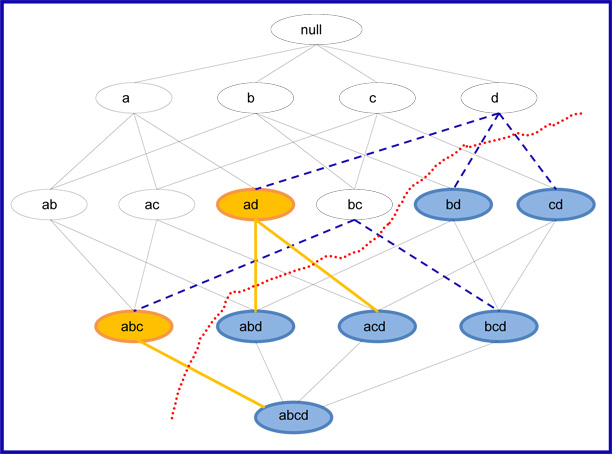
\includegraphics[width=\linewidth]{figures/maxFISExample}
  \caption{Maximal Frequent Itemset Illustration}
  \label{fig:maxFISExample}
\end{figure}


\paragraph{Closed Frequent Itemset }
It is a frequent itemset that is both closed and its support is greater than or equal to minsup.
An itemset is closed in a data set if there exists no superset that has the same support count as this original itemset.
Figure \ref{fig:closedFISExample} shows the maximal, closed and frequent itemsets. The itemsets that are circled with blue are the frequent itemsets. The itemsets that are circled with the thick blue are the closed frequent itemsets. The itemsets that are circled with the thick blue and have the yellow fill are the maximal frequent itemsets. In order to determine which of the frequent itemsets are closed, all you have to do is check to see if they have the same support as their supersets, if they do they are not closed.
For example \textbf{ad} is a frequent itemset but has the same support as \textbf{abd} so it is NOT a closed frequent itemset; \textbf{c} on the other hand is a closed frequent itemset because all of its supersets, \textbf{ac, bc}, and \textbf{cd} have supports that are less than 3.
As we can see there are a total of 9 frequent itemsets, 4 of them are closed frequent itemsets and out of these 4, 2 of them are maximal frequent itemsets. This brings us to the relationship between the three representations of frequent itemsets.

\begin{figure}
  \centering
  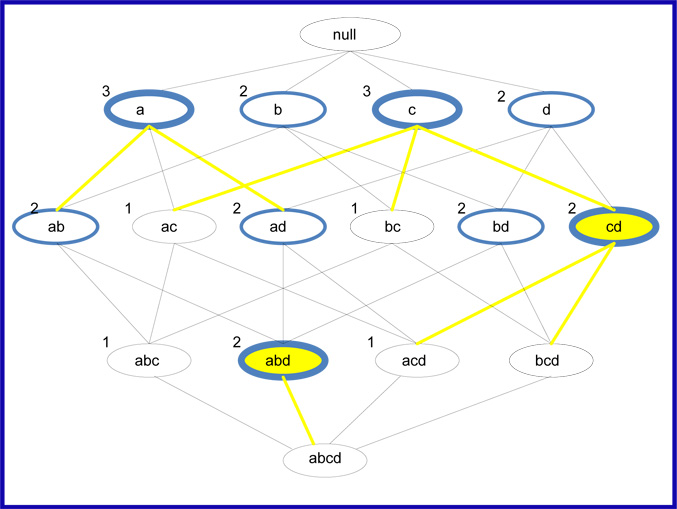
\includegraphics[width=\linewidth]{figures/closedFISExample}
  \caption{Maximal Frequent Itemset Illustration}
  \label{fig:closedFISExample}
\end{figure}


Figure ~\ref{fig:relationBetweenFIS} demonstrates the relations between the 
\begin{figure}
  \centering
  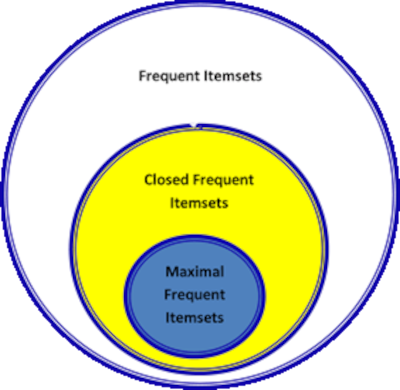
\includegraphics[width=\linewidth]{figures/relationBetweenFIS}
  \caption{Relationship between Frequent Itemset Representations}
  \label{fig:relationBetweenFIS}
\end{figure}

\subsection{FP-Tree and FP-Growth}
\paragraph{Apriori}
One of the earliest and most well known algorithms for mining association rules is the Apriori algorithm~\cite{agrawal1994fast}. This algorithm is iteratively generating candidates and pruning items with low support at each step. The correctness of this algorithm is based on the prove that if an item of length N is frequent, then all sub patterns must be frequent as well. Using that idea, an early prune of non-frequent itemsets removes many unnecessary candidates in later iterations. An example is provided in \autoref{fig:aprioriexample}. We will not expand further this algorithm, but this algorithm is intuitive and widely used. We would also mention that this algorithm main limitation is the candidate generation at every iteration, where many candidates may not be relevant and this information could have already used in previous stages.
  

\paragraph{FPGrowth}
In the year 2000, a tree based solution was introduced, FPGrowth algorithm and the FP-Tree structure~\cite{agrawal1994fast}. This algorithm removes the need for candidate generation and yields better performance~\cite{hunyadi2011performance}. 

TODO: Add algo
A small example is provided in \autoref{fig:fpgrowthexample}

\begin{figure}
  \centering
  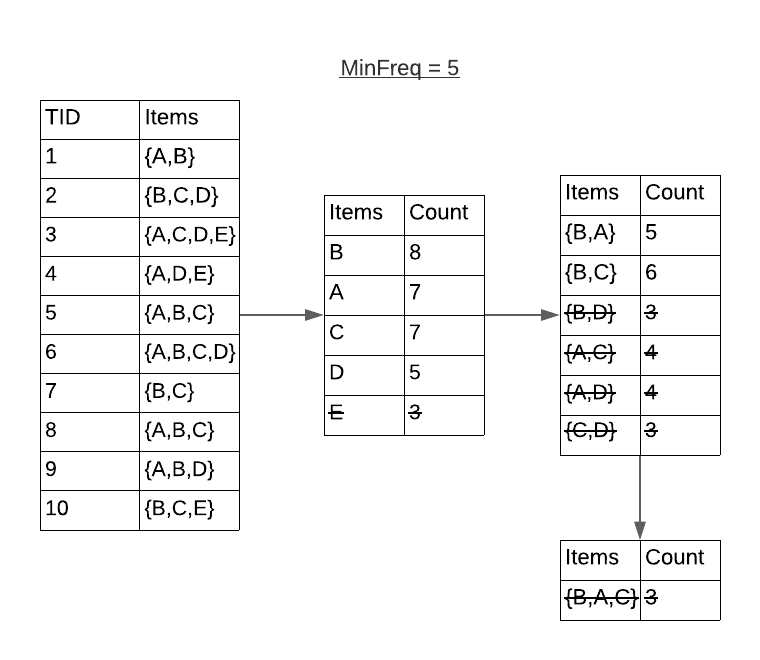
\includegraphics[width=\linewidth]{figures/aprioriexample}
  \caption{Apriori Example}
  \label{fig:aprioriexample}
\end{figure}

\begin{figure}
  \centering
  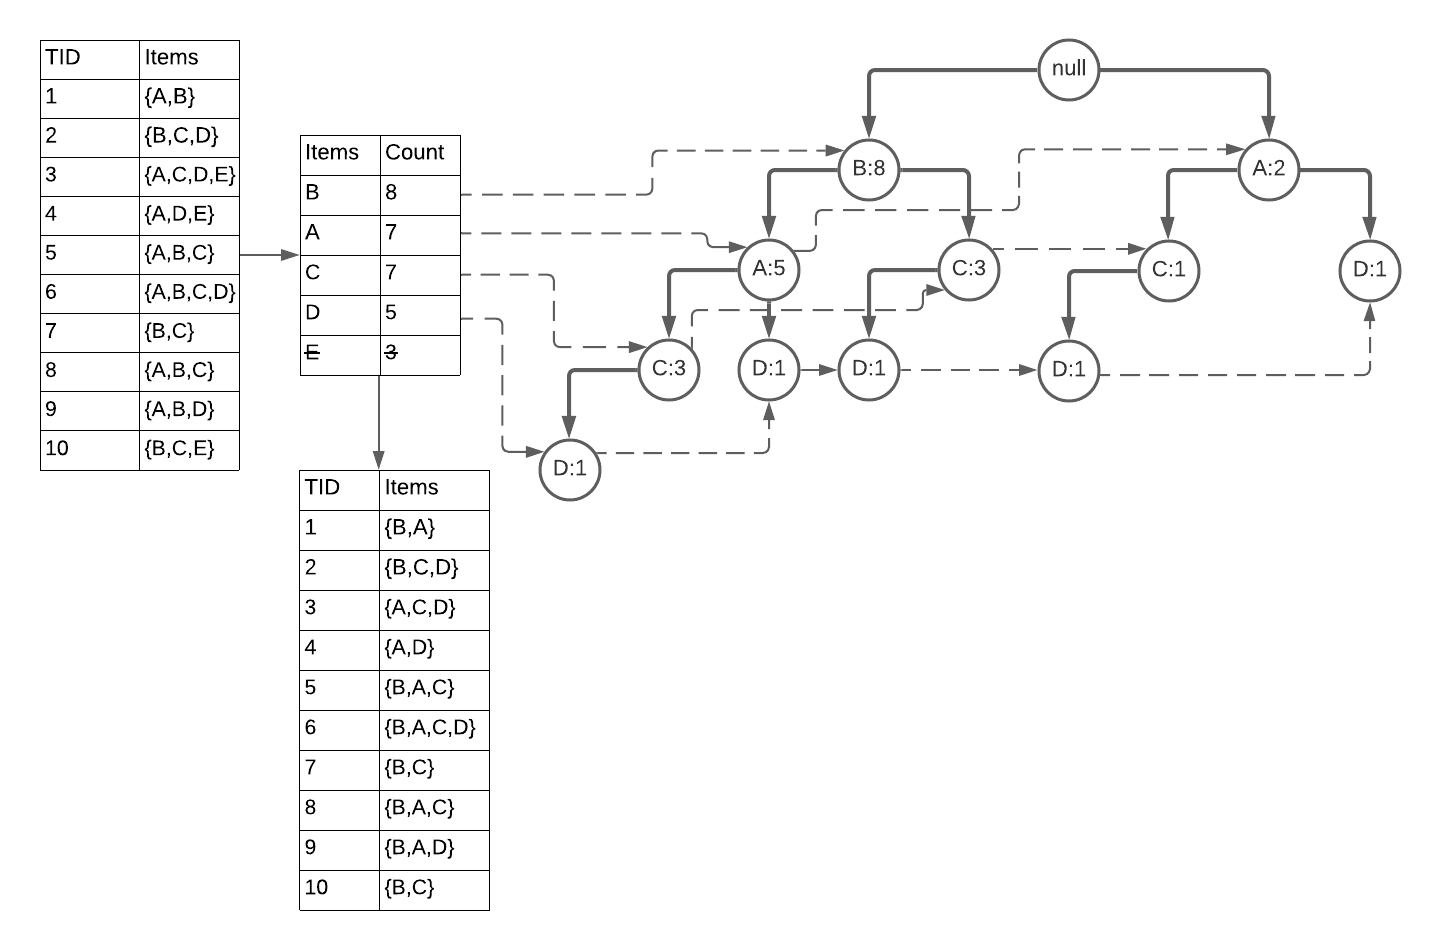
\includegraphics[width=\linewidth]{figures/FPTree}
  \caption{FPGrowth example}
  \label{fig:fpgrowthexample}
\end{figure}

\subsection{Apache Spark vs Hadoop}
\label{sec:sparkvhadoop}
The work by Daniele Apiletti et el. ~\cite{APILETTI201767} is focusing on comparing different frequent itemset mining algorithms between the Apache Hadoop ~\cite{hadoop} and Apache Spark ~\cite{spark}.

This work is performing extensive evaluation on synthetic and real world datasets and testing execution time, load balancing, and communication costs between 4 parallel itemset mining algorithm.

The participating algorithms are:
\begin{enumerate}
\item The Parallel FP-Growth implementation provided in Hadoop  Mahout 0.9 ~\cite{mahoot}
\item The Parallel FP-Growth implementation provided in MLlib for Spark
1.3.0 ~\cite{mllib}
\item The June 2015 implementation of BigFIM ~\cite{bigfim} 
\item The version of DistEclat downloaded from ~\cite{bigfim} on September 2015
\end{enumerate}
In our work we are using as the infrastructure, the PFP implementation of the MLLib ~\cite{mllib}  library in Spark,  which is one of the evaluated algorithms in the article ~\cite{APILETTI201767}.

BigFIM and DistEclat are not relevant to this work.

On page 27, the article mentions that except the Spark MLLib PFP~\cite{mllib} algorithm, all other implementations are mining closed itemsets,  and thus to obtain the
same output, the execution times of Mahout PFP, BigFIM and DistEclat may increase
with respect to MLlib PFP.

The evaluations in the paper were done using synthetic and real-world data.
The synthetic data and real-world data 
The results of the paper tested a synthetic and real-world data 



\begin{figure}
  \centering
  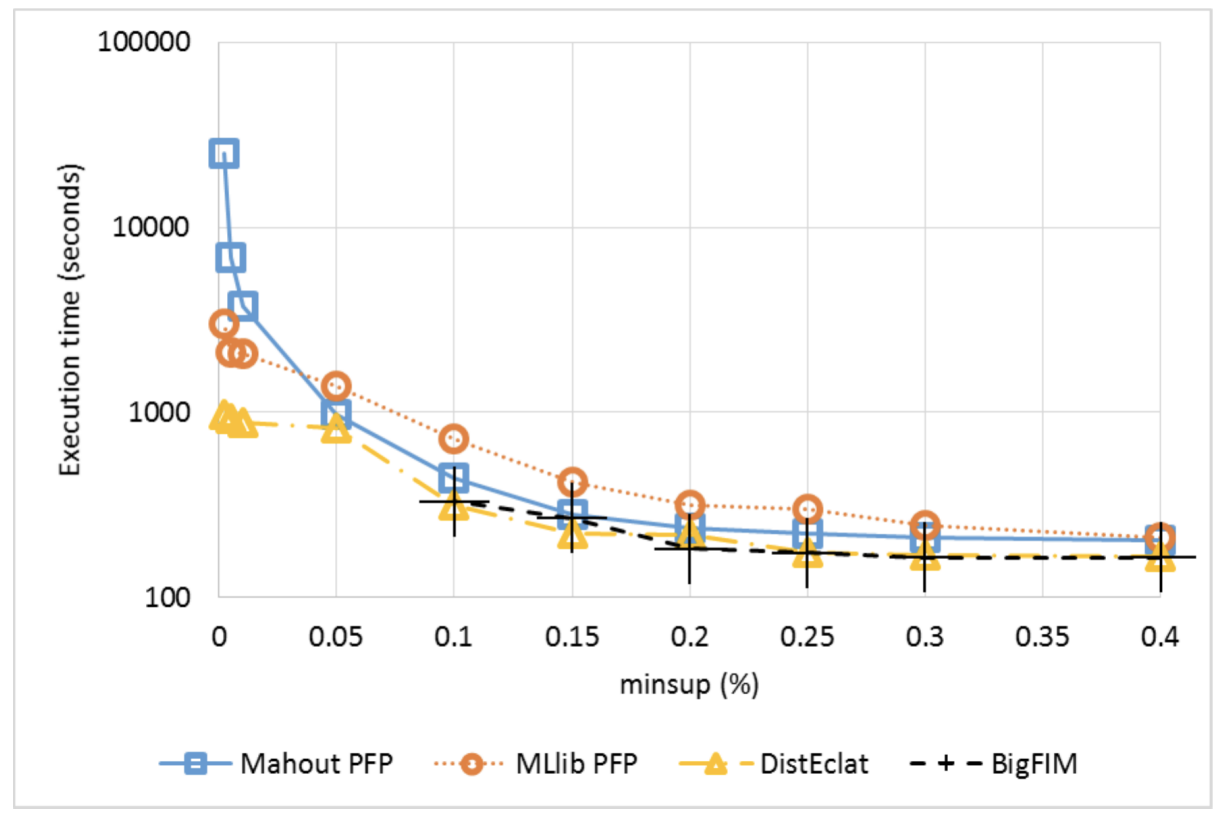
\includegraphics[width=\linewidth]{figures/sparkVsHadoopfig6}
  \caption{Execution time for different min-sup values, average transaction length 10}
  \label{fig:sparkVsHadoopfig6}
\end{figure}

\begin{figure}
  \centering
  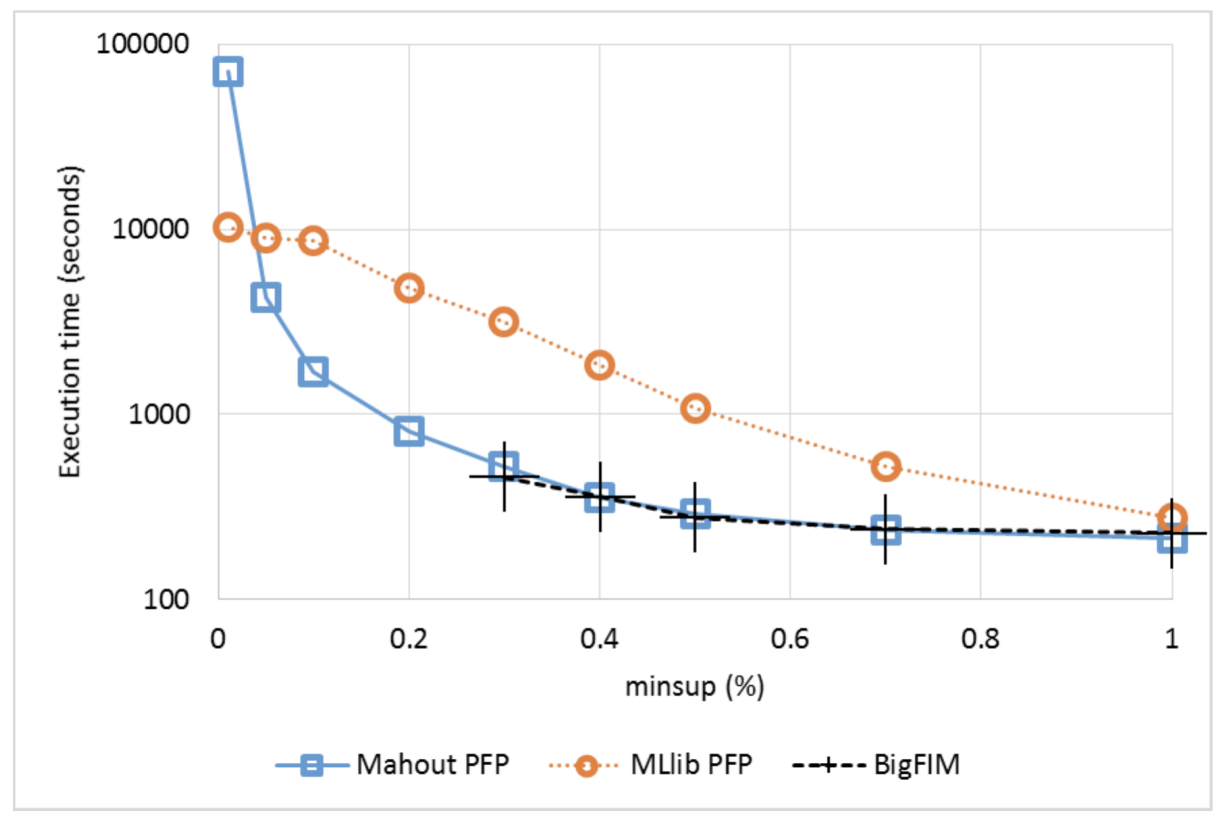
\includegraphics[width=\linewidth]{figures/sparkVsHadoopfig7}
  \caption{ Execution time for different min-sup values , average transaction length 30}
  \label{fig:sparkVsHadoopfig7}
\end{figure}
